\documentclass[]{exam} % {{{
\usepackage{amsmath, amssymb, amsthm, mathtools}
\usepackage{tikz, float, tabu, enumitem, hyperref}
\usetikzlibrary{calc,decorations.markings,matrix,arrows,positioning}

\usepackage{graphics}
\usepackage{circuitikz}

\usepackage{alltt}
%\usepackage{algorithm}
\usepackage[linesnumbered,ruled,vlined]{algorithm2e} 
\DeclareMathOperator*{\argmin}{argmin}
\DeclareMathOperator*{\argmax}{argmax}
\DeclareMathOperator*{\D}{\mathcal{D}}
\DeclareMathOperator*{\X}{\mathcal{X}}
\DeclareMathOperator*{\Hy}{\mathcal{H}}

% true or false questions (use \TFQuestion)
\newcommand{\TrueFalse}{\hspace*{0.25em}\textbf{True}\hspace*{1.25em}\textbf{False}\hspace*{1em}}
\newlength{\mylena} \newlength{\mylenb}
\settowidth{\mylena}{\TrueFalse}
\newcommand{\TFQuestion}[1]{
  \setlength{\mylenb}{\linewidth} 
  \addtolength{\mylenb}{-121.15pt}
  \parbox[t]{\mylena}{\TrueFalse}\parbox[t]{\mylenb}{#1}}

% document specific stuff
\pagestyle{foot}
\cfoot{Page \thepage\ of \numpages}

%============================================================================}}}

\begin{document}
% quiz header  {{{
\noindent\textbf{\large{EECS 738/800: Homework 4}} \hfill 2017-04-12
\smallskip
\hrule 
\bigskip
Name: Elise McEllhiney \qquad
Collaborators: David Young, David M\'enager, Bekah Coggins

\bigskip
%\noindent \textbf{Name:} \underline{\hspace{200pt}}
\medskip

\begin{questions} %\printanswers
%SVM 1 From the AML sup. chapter{{{
\question Consider the data below and a `hyperplane' $(b, \mathbf{w})$ that
separates the data.

\begin{align*}
   X = 
  \begin{bmatrix} 
  0 & 0 \\
  2 & 2 \\
  2 & 0 \\
  \end{bmatrix} 
  \hspace{2em}
   &y = 
  \begin{bmatrix} 
  -1 \\
  -1 \\
  +1 \\
  \end{bmatrix} 
  \hspace{2em}
   \mathbf{w} = 
  \begin{bmatrix} 
  1.2  \\
  -3.2 \\
  \end{bmatrix} 
  \hspace{2em}
  b = -0.5
\end{align*}
\begin{parts}
\part Compute $\rho = \min_{i=1,\ldots,N} y_i (\mathbf{w}^T\mathbf{x}_i + b)$.

\begin{align}
\rho 
& = \min_{i=1,\ldots,N} 
\begin{bmatrix}
  -1 \\
  -1 \\
  +1 \\
\end{bmatrix}
\Big(
\begin{bmatrix} 
  1.2  & -3.2 
\end{bmatrix} 
\begin{bmatrix} 
  0 & 0 \\
  2 & 2 \\
  2 & 0 \\
\end{bmatrix}
+ (-0.5) \Big) \\
& = \min_{i=1,\ldots,N} 
\begin{bmatrix}
  -1 \\
  -1 \\
  +1 \\
\end{bmatrix}
 \Big(
\begin{bmatrix} 
  0 \\
  -4 \\
  2.4 \\
\end{bmatrix}
+ (-0.5) \Big) \\
& = \min_{i=1,\ldots,N} 
\begin{bmatrix}
  -1 \\
  -1 \\
  +1 \\
\end{bmatrix}
\begin{bmatrix} 
  -0.5 \\
  -4.5 \\
  1.9 \\
\end{bmatrix} \\
& = \min_{i=1,\ldots,N} 
\begin{bmatrix} 
  0.5 \\
  4.5 \\
  1.9 \\
\end{bmatrix} \\
\rho & = 0.5
\end{align}

\part Compute the weights $\frac{1}{\rho}(b,\mathbf{w})$ and show that they satisfy $\min_{i=1,\ldots,N} y_i (\mathbf{w}^T\mathbf{x}_i + b) = 1$.

\begin{align} 
\min_{i=1,\ldots,N} 
\begin{bmatrix}
  -1 \\
  -1 \\
  +1 \\
\end{bmatrix}
 \Big(
\begin{bmatrix} 
  2.4  & -6.4 
\end{bmatrix} 
\begin{bmatrix} 
  0 & 0 \\
  2 & 2 \\
  2 & 0 \\
\end{bmatrix}
+ (-1) \Big)
& = \min_{i=1,\ldots,N} 
\begin{bmatrix}
  -1 \\
  -1 \\
  +1 \\
\end{bmatrix}
 \Big(
\begin{bmatrix} 
  0 \\
  -8 \\
  4.8 \\
\end{bmatrix}
+ (-1) \Big) \\
& = \min_{i=1,\ldots,N} 
\begin{bmatrix}
  -1 \\
  -1 \\
  +1 \\
\end{bmatrix}
\begin{bmatrix} 
  -1 \\
  -9 \\
  3.8 \\
\end{bmatrix} \\
& = \min_{i=1,\ldots,N} 
\begin{bmatrix} 
  1 \\
  9 \\
  3.8 \\
\end{bmatrix} \\
& = 1
\end{align}
\end{parts}
%}}}
%SVM 1 From ISLR {{{
\question Here we explore the maximal margin classifier (linearly separable SVM) on a toy data set.
\begin{parts}
\part We are given $n=7$ observations in $p=2$ dimensions. For each
observation, there is an associated class label.

\begin{center}
\begin{tabular} {c c c l}
\hline
Obs & $X_1$ & $X_2$ & $y$ \\
\hline
1 & 3 & 4 & Red \\
2 & 2 & 2 & Red \\
3 & 4 & 4 & Red \\
4 & 1 & 4 & Red \\
5 & 2 & 1 & Blue \\
6 & 4 & 3 & Blue \\
7 & 4 & 1 & Blue \\
\end{tabular}
\end{center}

Sketch the observations.

\begin{center}
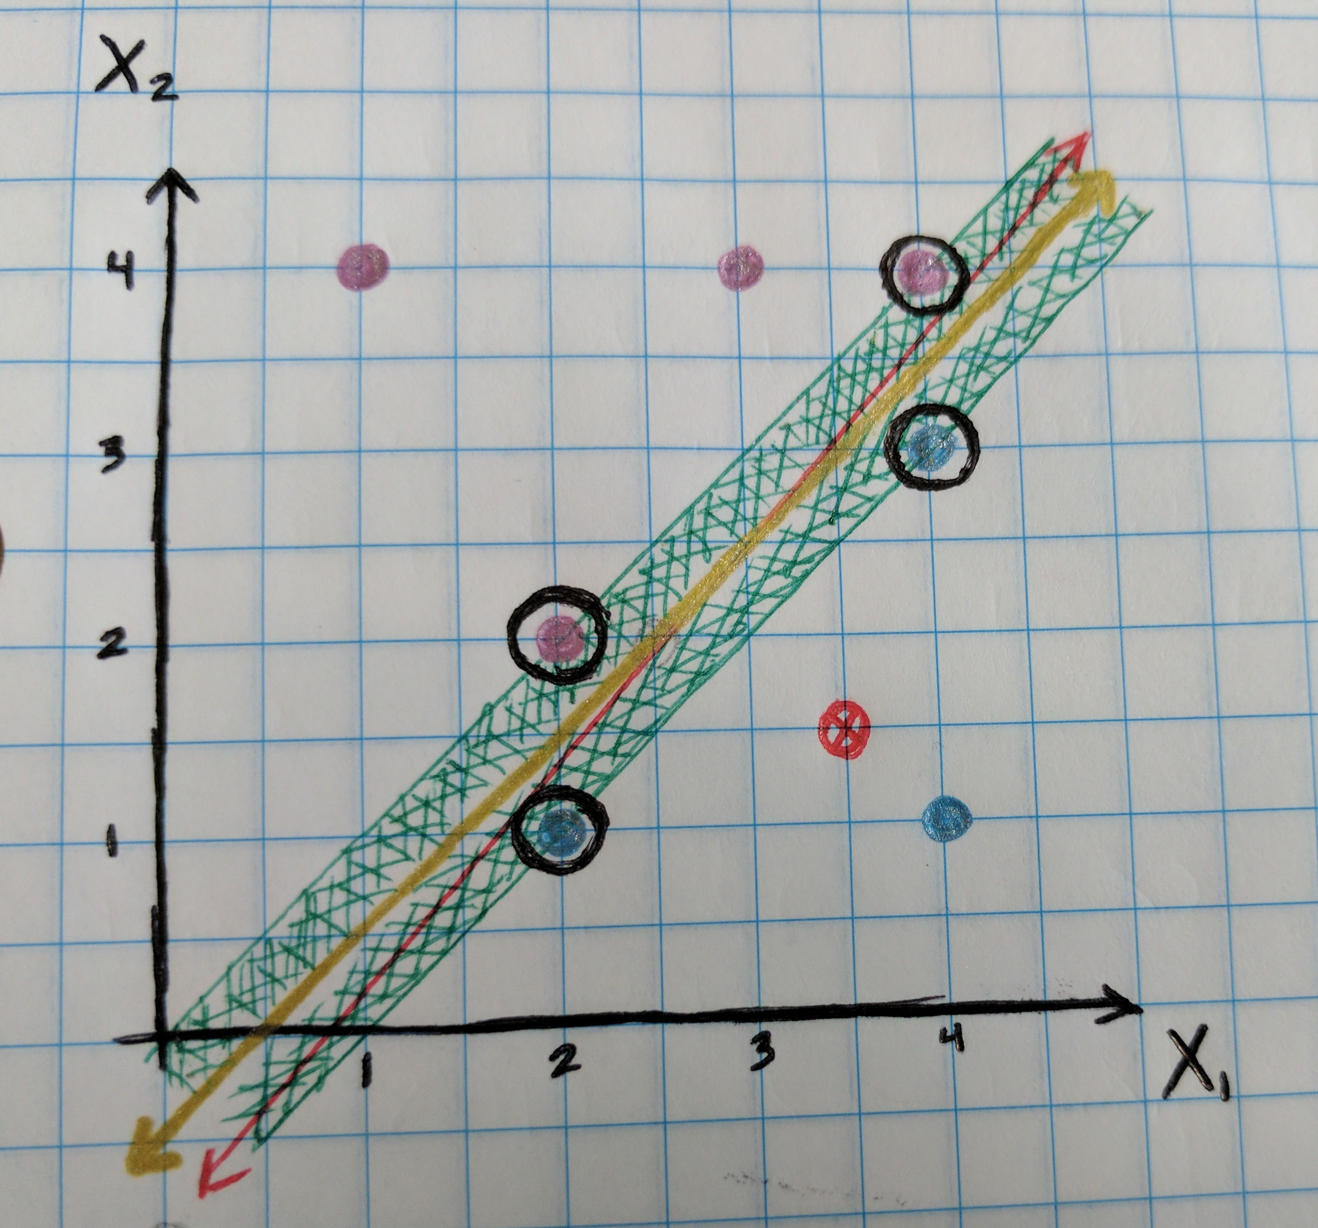
\includegraphics[width=10cm]{blah}
\end{center}

\part Sketch the optimal separating hyperplane and provide the equation for this hyperplane of the form $b+w_1 X_1 + w_2 X_2 = 0$.

\begin{align}
b + w_1 X_1 + w_2 X_2 & = 0 \\
-0.5 + X_1 - X_2 & = 0
\end{align}

\part Describe the classification rule for maximal margin (linear SVM) classifier. It should be something like "Classify to Red if $b+w_1 X_1 + w_2 X_2 \geq 0$ and classify to Blue otherwise. Provide $\mathbf{w}$ and $b$.

\begin{align}
b & = -0.5 \\
\pmb{w} & = [1,-1]
\end{align}
Classify to Red if $-0.5 + X_1 - X_2 \leq 0$ and to Blue otherwise.

\part On your sketch from the first part, indicate the margin for the hyperplane.

The margin is the green region

\part Indicate the support vectors for the classifier.

The support vectors are the circled points.

\part Argue that a slight movement of the seventh observation would or would not affect the hyperplane of our linear SVM.

Any point besides the support vectors will not effect the hyperplane by moving unless the movement causes the point to enter the margin or cross the hyperplane.  The point entering the margin would change the ideal hyperplane and reduce our margin since the point would become a support vector by being that close to the separating hyperplane.  Crossing the hyperplane would cause the point to be misclassified.  So for the 7th observation, it would have to move more than 3 units in one or both axis before it would even touch the margin.  So any deviation less than this wouldn't affect the hyperplane.

\part Sketch a hyperplane that separates the data but is not the optimal hyperplane. Provide an equation for this hyperplane.

The thin bright red line is a non-optimal hyperplane.
$$-5 + 6 X_1 - 5 X_2 = 0$$

\part Draw an additional observation on the plot so that the two classes are no longer separable by a hyperplane. Clearly label that point.

The bright red XOR symbol, if classified as "Red" would prevent the observations from being separable

\end{parts}
%}}}
% PCA vs LDA {{{
\question Principal Component Analysis (PCA) and Linear Discriminant 
Analysis (LDA) can both be used for dimensionality reduction.
\begin{parts}
\part Explain what the first principal component from PCA captures.

The first component from PCA is the eigenvector that captures the greatest variance.

\part How does PCA differ from LDA?

PCA determines component axes that maximize the variance.  These new axis are then used for class separation.  LDA, on the other hand, only maximizes the existing component axes for class separation.

\part Give a short description of why PCA can be used for image compression without much loss of image quality.

In image compression, PCA can be used without much loss in quality since past a reasonable number of principal components, the variance explained by additional components would not produce a notable change in the image.

\end{parts}
%}}}
%Neural Network question {{{
%http://www.cs.cmu.edu/~tom/10601_fall2012/hw/hw3_solutions.pdf
\question Neural networks with a single hidden unit and a logistic activation function have real-valued inputs $X_1, \ldots, X_n$ where the unit output $Y$ is defined as
\[ Y = \frac{1}{1+\text{exp}(-(w_0 + \sum_i w_i X_i))}. \]
Let the $X_i$ be either 0 or 1. We will assume that a value for $Y> 0.5$ is 1 and zero otherwise. So even though our neural network returns a probability, we will convert the probability to a 0 or 1.

\begin{parts}
\part Give 3 weights for a single unit with two inputs $X_1$ and $X_2$, that implements the logical ``OR'' function $Y= X_1 \vee X_2$.

Yes, this can be implemented in a single unit.

$$\pmb{w} = [-1, 2, 2] $$

\part Can you implement the logical ``AND'' function $Y= X_1 \wedge X_2$ with a single hidden unit? If so give weights that achieve this. If not, explain the problem.

Yes, this can be implemented in a single unit.

$$\pmb{w} = [-3, 2, 2] $$

\part Can you implement the logical ``EXCLUSIVE-OR'' function $Y= X_1 \bigoplus X_2$ with a single hidden unit? If so give weights that achieve this. If not, how many hidden units would you need?

No, this cannot be implemented with a single unit.  You would need two hidden units.  I assume that outputs of the neural units are 1 or 0.

\begin{center}
\begin{circuitikz} \draw
(0,4) node (x){x}
(1,4) node (y){y}
(3,2) node[and port] (and) {}
(3,0) node[nor port] (nor) {}
(5,1) node[nor port] (norOut) {}

(x) |- (and.in 1)
(x) |- (nor.in 1)
(y) |- (and.in 2)
(y) |- (nor.in 2)
(and.out) -- (norOut.in 1)
(nor.out) -- (norOut.in 2);
\end{circuitikz}
\end{center}

\begin{align}
\text{Hidden unit 1:} \quad \pmb{w} & = [-3, 2, 2] \\
\text{HIdden unit 2:} \quad \pmb{w} & = [1, -2, -2]\\
\text{Output node:} \quad \pmb{w} & = [1, -2, -2]
\end{align}
\end{parts}



%}}}
\end{questions}
\end{document}
